\documentclass{standalone}
\usepackage{tikz}
\usetikzlibrary{patterns, positioning}
\usepackage[sfdefault]{ClearSans} %% option 'sfdefault' activates Clear Sans as the default text font
\usepackage[T1]{fontenc}

\begin{document}
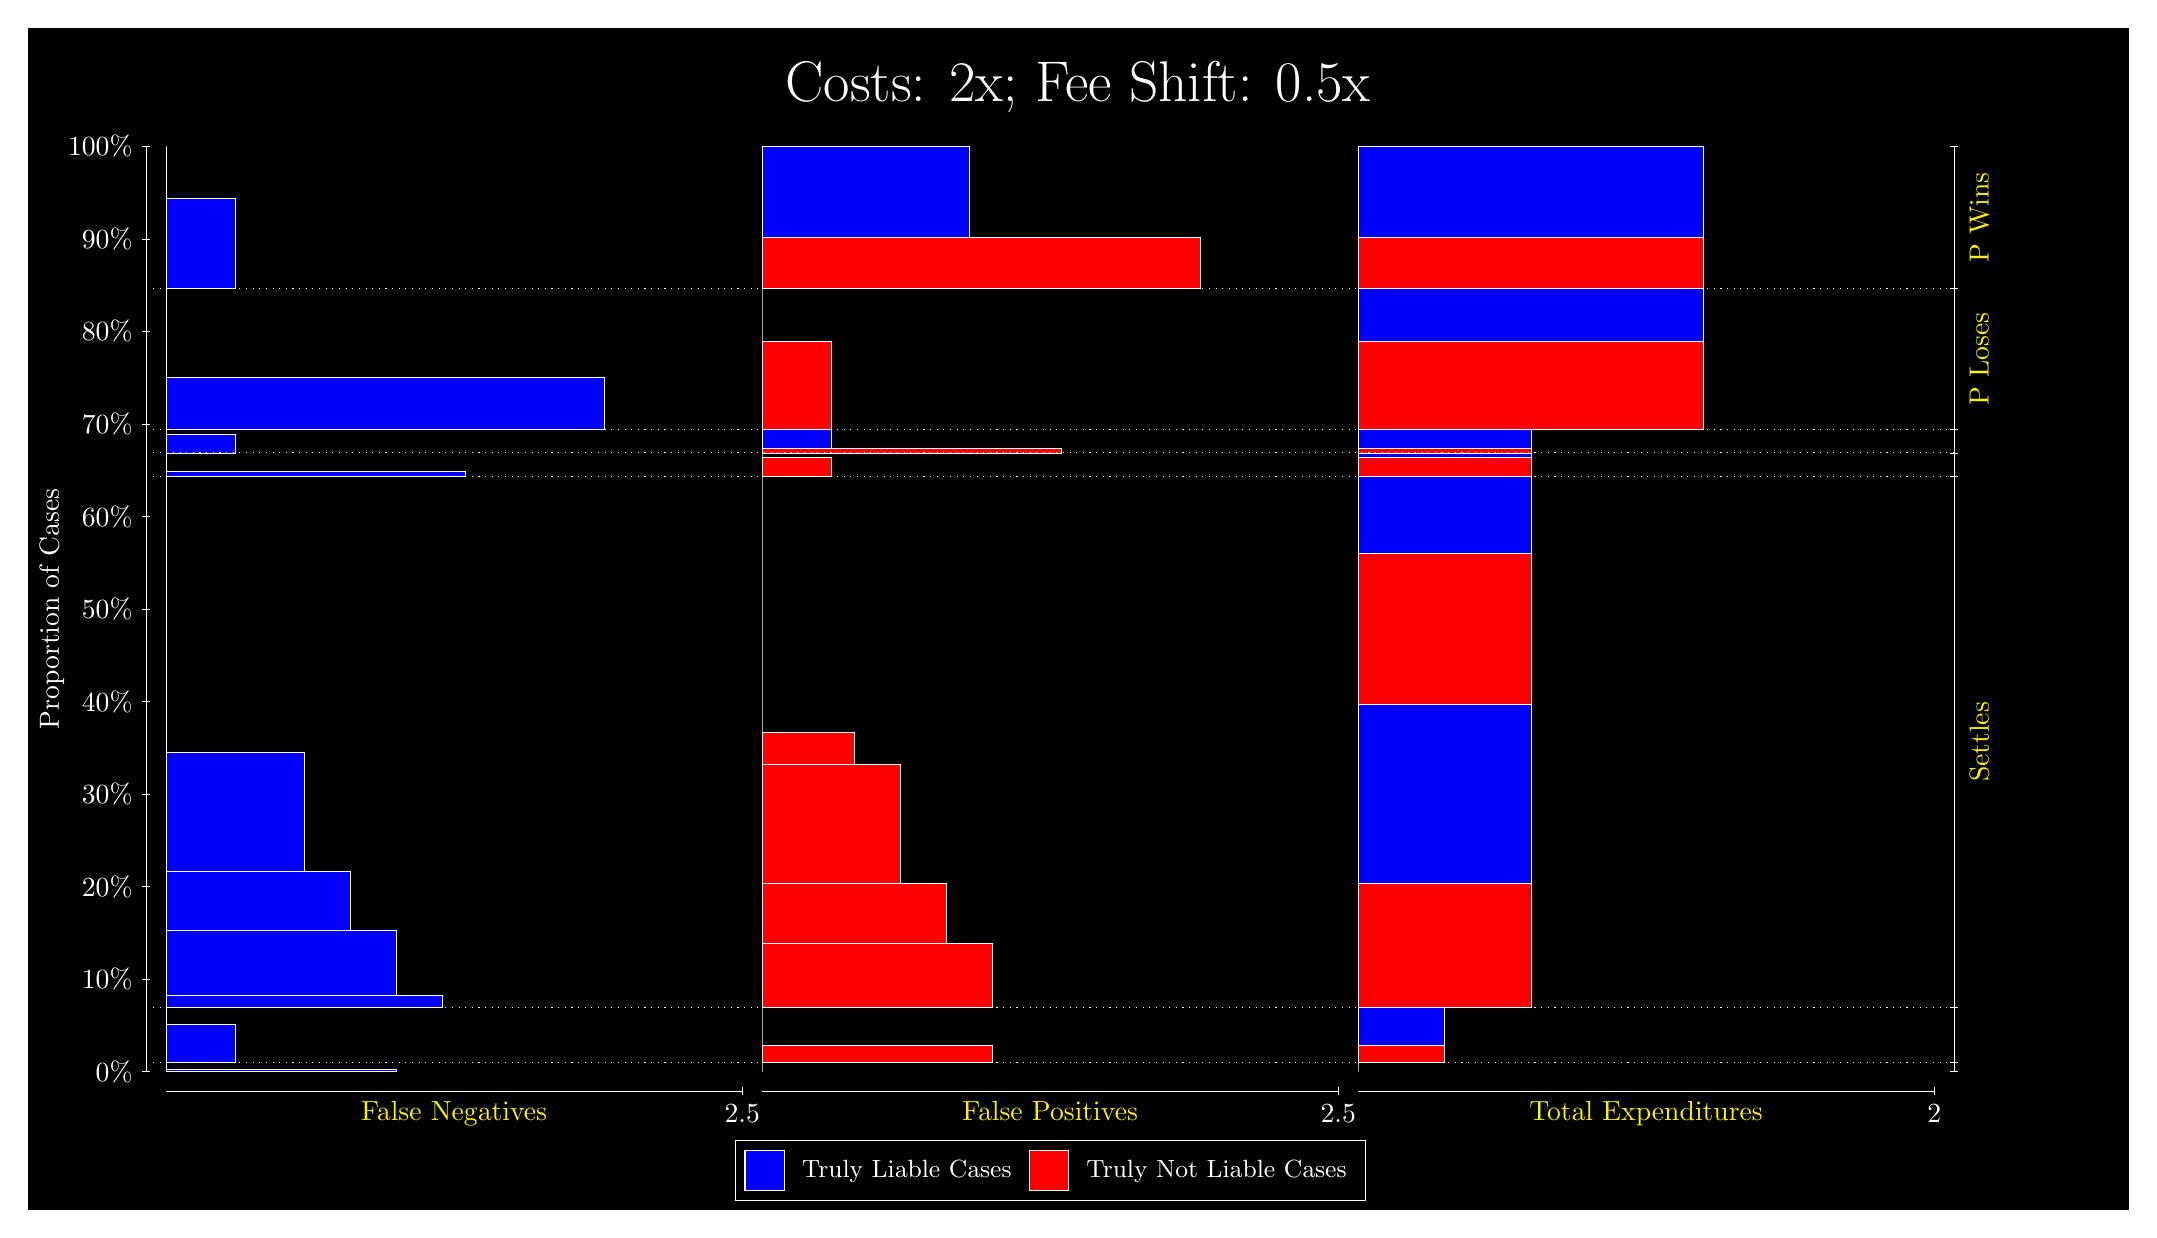
\begin{tikzpicture}
\draw[fill=black] (0,0) rectangle (26.667,15);
\draw[text=white] (0,13.5) rectangle (26.667,15) node[midway] {\huge Costs: 2x; Fee Shift: 0.5x};
\draw[white, very thin] (1.5,1.75) -- (1.5,13.5);
\node[rotate=90, text=white, anchor=center] at (0.3, 7.625) {Proportion of Cases};
\draw[white, very thin] (1.45,1.75) -- (1.55,1.75);
\node[text=white, anchor=east] at (1.45, 1.75) {0\%};
\draw[white, very thin] (1.45,2.925) -- (1.55,2.925);
\node[text=white, anchor=east] at (1.45, 2.925) {10\%};
\draw[white, very thin] (1.45,4.1) -- (1.55,4.1);
\node[text=white, anchor=east] at (1.45, 4.1) {20\%};
\draw[white, very thin] (1.45,5.275) -- (1.55,5.275);
\node[text=white, anchor=east] at (1.45, 5.275) {30\%};
\draw[white, very thin] (1.45,6.45) -- (1.55,6.45);
\node[text=white, anchor=east] at (1.45, 6.45) {40\%};
\draw[white, very thin] (1.45,7.625) -- (1.55,7.625);
\node[text=white, anchor=east] at (1.45, 7.625) {50\%};
\draw[white, very thin] (1.45,8.8) -- (1.55,8.8);
\node[text=white, anchor=east] at (1.45, 8.8) {60\%};
\draw[white, very thin] (1.45,9.975) -- (1.55,9.975);
\node[text=white, anchor=east] at (1.45, 9.975) {70\%};
\draw[white, very thin] (1.45,11.15) -- (1.55,11.15);
\node[text=white, anchor=east] at (1.45, 11.15) {80\%};
\draw[white, very thin] (1.45,12.325) -- (1.55,12.325);
\node[text=white, anchor=east] at (1.45, 12.325) {90\%};
\draw[white, very thin] (1.45,13.5) -- (1.55,13.5);
\node[text=white, anchor=east] at (1.45, 13.5) {100\%};

\draw[white, very thin] (24.457,1.75) -- (24.457,13.5);
\draw[white, very thin] (24.407,1.75) -- (24.507,1.75);
\node[anchor=west] at (24.407, 1.75) {};
\draw[white, very thin] (24.407,1.8667) -- (24.507,1.8667);
\node[anchor=west] at (24.407, 1.8667) {};
\draw[white, very thin] (24.407,2.5639) -- (24.507,2.5639);
\node[anchor=west] at (24.407, 2.5639) {};
\draw[white, very thin] (24.407,9.3085) -- (24.507,9.3085);
\node[anchor=west] at (24.407, 9.3085) {};
\draw[white, very thin] (24.407,9.6062) -- (24.507,9.6062);
\node[anchor=west] at (24.407, 9.6062) {};
\draw[white, very thin] (24.407,9.9039) -- (24.507,9.9039);
\node[anchor=west] at (24.407, 9.9039) {};
\draw[white, very thin] (24.407,11.691) -- (24.507,11.691);
\node[anchor=west] at (24.407, 11.691) {};
\draw[white, very thin] (24.407,13.5) -- (24.507,13.5);
\node[anchor=west] at (24.407, 13.5) {};

\draw[white, very thin, fill=blue] (1.75,1.75) rectangle (4.6775,1.782);
\draw[white, very thin, fill=red] (1.75,1.782) rectangle (1.75,1.8667);
\draw[white, very thin, fill=blue] (1.75,1.8667) rectangle (2.6283,2.3462);
\draw[white, very thin, fill=red] (1.75,2.3462) rectangle (1.75,2.5639);
\draw[white, very thin, fill=blue] (1.75,2.5639) rectangle (5.2631,2.7202);
\draw[white, very thin, fill=blue] (1.75,2.7202) rectangle (4.6775,3.5377);
\draw[white, very thin, fill=blue] (1.75,3.5377) rectangle (4.092,4.2913);
\draw[white, very thin, fill=blue] (1.75,4.2913) rectangle (3.5065,5.8107);
\draw[white, very thin, fill=red] (1.75,5.8107) rectangle (1.75,9.3085);
\draw[white, very thin, fill=blue] (1.75,9.3085) rectangle (5.5558,9.3668);
\draw[white, very thin, fill=red] (1.75,9.3668) rectangle (1.75,9.6062);
\draw[white, very thin, fill=blue] (1.75,9.6062) rectangle (2.6283,9.8456);
\draw[white, very thin, fill=red] (1.75,9.8456) rectangle (1.75,9.9039);
\draw[white, very thin, fill=blue] (1.75,9.9039) rectangle (7.3123,10.571);
\draw[white, very thin, fill=red] (1.75,10.571) rectangle (1.75,11.691);
\draw[white, very thin, fill=blue] (1.75,11.691) rectangle (2.6283,12.843);
\draw[white, very thin, fill=red] (1.75,12.843) rectangle (1.75,13.5);
\draw[white, very thin, fill=red] (9.3189,1.75) rectangle (9.3189,1.8347);
\draw[white, very thin, fill=blue] (9.3189,1.8347) rectangle (9.3189,1.8667);
\draw[white, very thin, fill=red] (9.3189,1.8667) rectangle (12.246,2.0844);
\draw[white, very thin, fill=blue] (9.3189,2.0844) rectangle (9.3189,2.5639);
\draw[white, very thin, fill=red] (9.3189,2.5639) rectangle (12.246,3.3813);
\draw[white, very thin, fill=red] (9.3189,3.3813) rectangle (11.661,4.135);
\draw[white, very thin, fill=red] (9.3189,4.135) rectangle (11.075,5.6543);
\draw[white, very thin, fill=red] (9.3189,5.6543) rectangle (10.49,6.0617);
\draw[white, very thin, fill=blue] (9.3189,6.0617) rectangle (9.3189,9.3085);
\draw[white, very thin, fill=red] (9.3189,9.3085) rectangle (10.197,9.5479);
\draw[white, very thin, fill=blue] (9.3189,9.5479) rectangle (9.3189,9.6062);
\draw[white, very thin, fill=red] (9.3189,9.6062) rectangle (13.125,9.6645);
\draw[white, very thin, fill=blue] (9.3189,9.6645) rectangle (10.197,9.9039);
\draw[white, very thin, fill=red] (9.3189,9.9039) rectangle (10.197,11.024);
\draw[white, very thin, fill=blue] (9.3189,11.024) rectangle (9.3189,11.691);
\draw[white, very thin, fill=red] (9.3189,11.691) rectangle (14.881,12.348);
\draw[white, very thin, fill=blue] (9.3189,12.348) rectangle (11.954,13.5);
\draw[white, very thin, fill=red] (16.888,1.75) rectangle (16.888,1.8347);
\draw[white, very thin, fill=blue] (16.888,1.8347) rectangle (16.888,1.8667);
\draw[white, very thin, fill=red] (16.888,1.8667) rectangle (17.986,2.0844);
\draw[white, very thin, fill=blue] (16.888,2.0844) rectangle (17.986,2.5639);
\draw[white, very thin, fill=red] (16.888,2.5639) rectangle (19.083,4.135);
\draw[white, very thin, fill=blue] (16.888,4.135) rectangle (19.083,6.408);
\draw[white, very thin, fill=red] (16.888,6.408) rectangle (19.083,8.3347);
\draw[white, very thin, fill=blue] (16.888,8.3347) rectangle (19.083,9.3085);
\draw[white, very thin, fill=red] (16.888,9.3085) rectangle (19.083,9.5479);
\draw[white, very thin, fill=blue] (16.888,9.5479) rectangle (19.083,9.6062);
\draw[white, very thin, fill=red] (16.888,9.6062) rectangle (19.083,9.6645);
\draw[white, very thin, fill=blue] (16.888,9.6645) rectangle (19.083,9.9039);
\draw[white, very thin, fill=red] (16.888,9.9039) rectangle (21.279,11.024);
\draw[white, very thin, fill=blue] (16.888,11.024) rectangle (21.279,11.691);
\draw[white, very thin, fill=red] (16.888,11.691) rectangle (21.279,12.348);
\draw[white, very thin, fill=blue] (16.888,12.348) rectangle (21.279,13.5);
\draw[white, dotted] (1.5,1.8667) -- (24.457,1.8667);
\draw[white, dotted] (1.5,2.5639) -- (24.457,2.5639);
\draw[white, dotted] (1.5,9.3085) -- (24.457,9.3085);
\draw[white, dotted] (1.5,9.6062) -- (24.457,9.6062);
\draw[white, dotted] (1.5,9.9039) -- (24.457,9.9039);
\draw[white, dotted] (1.5,11.691) -- (24.457,11.691);
\draw[white, very thin] (1.75,1.5) -- (9.0689,1.5);
\node[text=yellow, anchor=north] at (5.4094, 1.5) {False Negatives};
\draw[white, very thin] (9.0689,1.45) -- (9.0689,1.55);
\node[text=white, anchor=north] at (9.0689, 1.45) {2.5};

\draw[white, very thin] (9.3189,1.5) -- (16.638,1.5);
\node[text=yellow, anchor=north] at (12.978, 1.5) {False Positives};
\draw[white, very thin] (16.638,1.45) -- (16.638,1.55);
\node[text=white, anchor=north] at (16.638, 1.45) {2.5};

\draw[white, very thin] (16.888,1.5) -- (24.207,1.5);
\node[text=yellow, anchor=north] at (20.547, 1.5) {Total Expenditures};
\draw[white, very thin] (24.207,1.45) -- (24.207,1.55);
\node[text=white, anchor=north] at (24.207, 1.45) {2};



\node[text=yellow, centered, rotate=90] at (24.777, 5.9362) {Settles};


\node[text=yellow, centered, rotate=90] at (24.777, 10.798) {P Loses};
\node[text=yellow, centered, rotate=90] at (24.777, 12.596) {P Wins};

\draw (12.978300999999998,1.5) node[draw=none] (baseCoordinate) {};
\begin{scope}[align=center]
        \matrix[scale=0.5, draw=white, below=0.5cm of baseCoordinate, nodes={draw}, column sep=0.1cm]{
            \node[rectangle, draw, minimum width=0.5cm, minimum height=0.5cm, fill=blue] {}; &
            \node[draw=none, font=\small, text=white] (B) {Truly Liable Cases}; &
            \node[rectangle, draw, minimum width=0.5cm, minimum height=0.5cm, fill=red] {}; &
            \node[draw=none, font=\small, text=white] (B) {Truly Not Liable Cases}; \\
            };
\end{scope}

\end{tikzpicture}
\end{document}